\documentclass[boxes]{gsypset}

% Info for header
\mailbox{}
\initials{}
\collaborators{}
\class{Math 60}
\assignment{HW 5}
\duedate{May 23, 2016}
\problemlist{3.3.24, 3.4.\{4, 7, 12, 13, 16, 23\}}

\DeclareMathOperator{\curl}{curl}
\DeclareMathOperator{\divergence}{div}

\begin{document}
\begin{problem}[3.3.24]
	Consider the vector field
	$\mathbf{F}=2x\mathbf{i}+2y\mathbf{j}-3\mathbf{k}$.
	\begin{subproblems}
		\subproblem
			Show that $\mathbf{F}$ is a gradient field.
			\begin{solution}
				
			\end{solution}
		\subproblem 
			Describe the equipotential surfaces of $\mathbf{F}$ in words and with sketches.
			\begin{solution}
				
			\end{solution}
	\end{subproblems}
\end{problem}

\begin{problem}[3.4.4]
	Calculate the divergence of the vector field
	\[
		\mathbf{F} = z\cos\left(e^{y^2}\right)\;\mathbf{i} + 
		             x\sqrt{z^2+1}\;\mathbf{j} + 
		             e^{2y}\sin3x\;\mathbf{k}
	\]
\end{problem}
\begin{solution}
	
\end{solution}

\begin{problem}[3.4.7]
	Find the curl of the vector field
	\[
		\mathbf{F} = x^2\;\mathbf{i} - xe^y\;\mathbf{j} + 2xyz\;\mathbf{k}
	\]
\end{problem}
\begin{solution}
	
\end{solution}

\begin{problem}[3.4.12]
	\begin{subproblems}
		\subproblem 
			Consider the vector field 
			$\mathbf{F} = x\mathbf{i} + y\mathbf{j} + z\mathbf{k}$ and its curl. 
			Sketch the vector field and use your picture to explain 
			geometrically why the curl is as we calculated in class.
			\begin{solution}
				
			\end{solution}
		\subproblem
			Use geometry to determine $\nabla\times\mathbf{F}$, where
			\[
				\mathbf{F} = \frac{(x\mathbf{i}+ y\mathbf{j} +z\mathbf{k})}{\sqrt{x^2+y^2+z^2}}
			\]
			\begin{solution}
				
			\end{solution}
		\subproblem
			For $\mathbf{F}$ as in part (b), verify your intuition by explicitly computing 
			$\nabla\times\mathbf{F}$.
			\begin{solution}
				
			\end{solution}
	\end{subproblems}
\end{problem}

\begin{problem}[3.4.13]
	Can you tell in what portions of $\mathbb{R}^2$, the vector fields shown
	in Figures 3.43-3.46 have positive divergence? Negative
	divergence?
	\begin{center}
		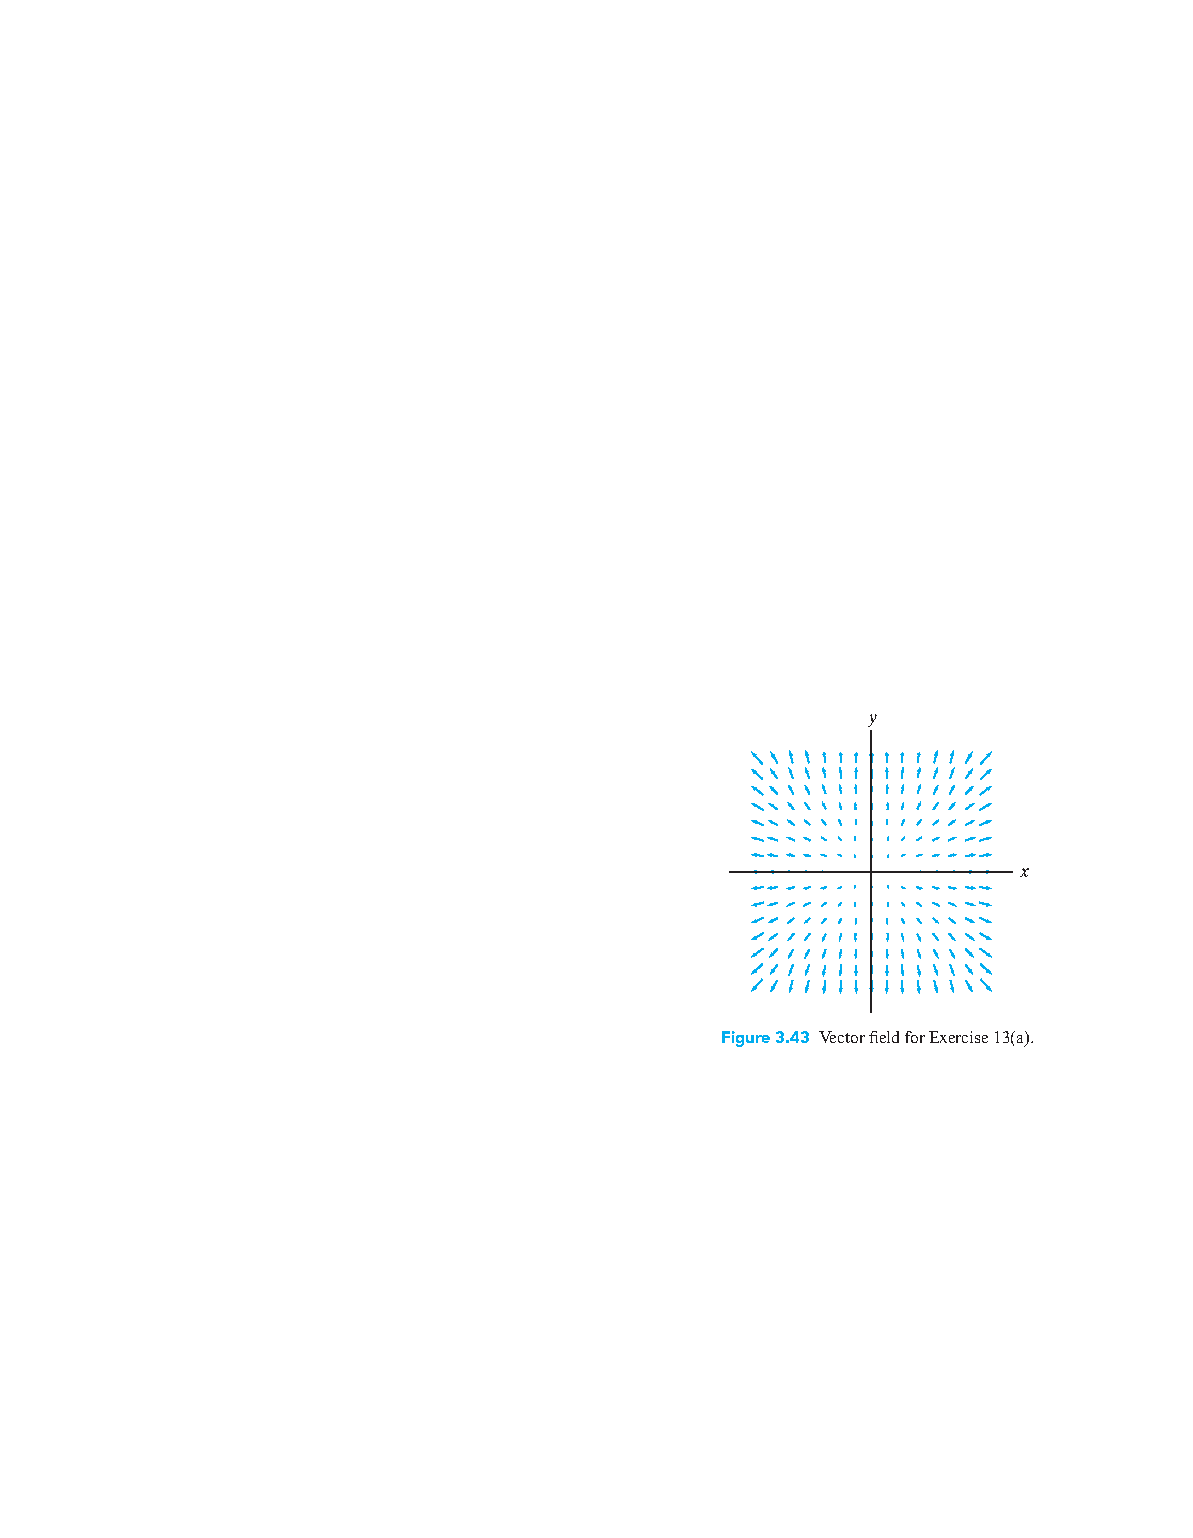
\includegraphics{img/3_4_13a}\qquad
		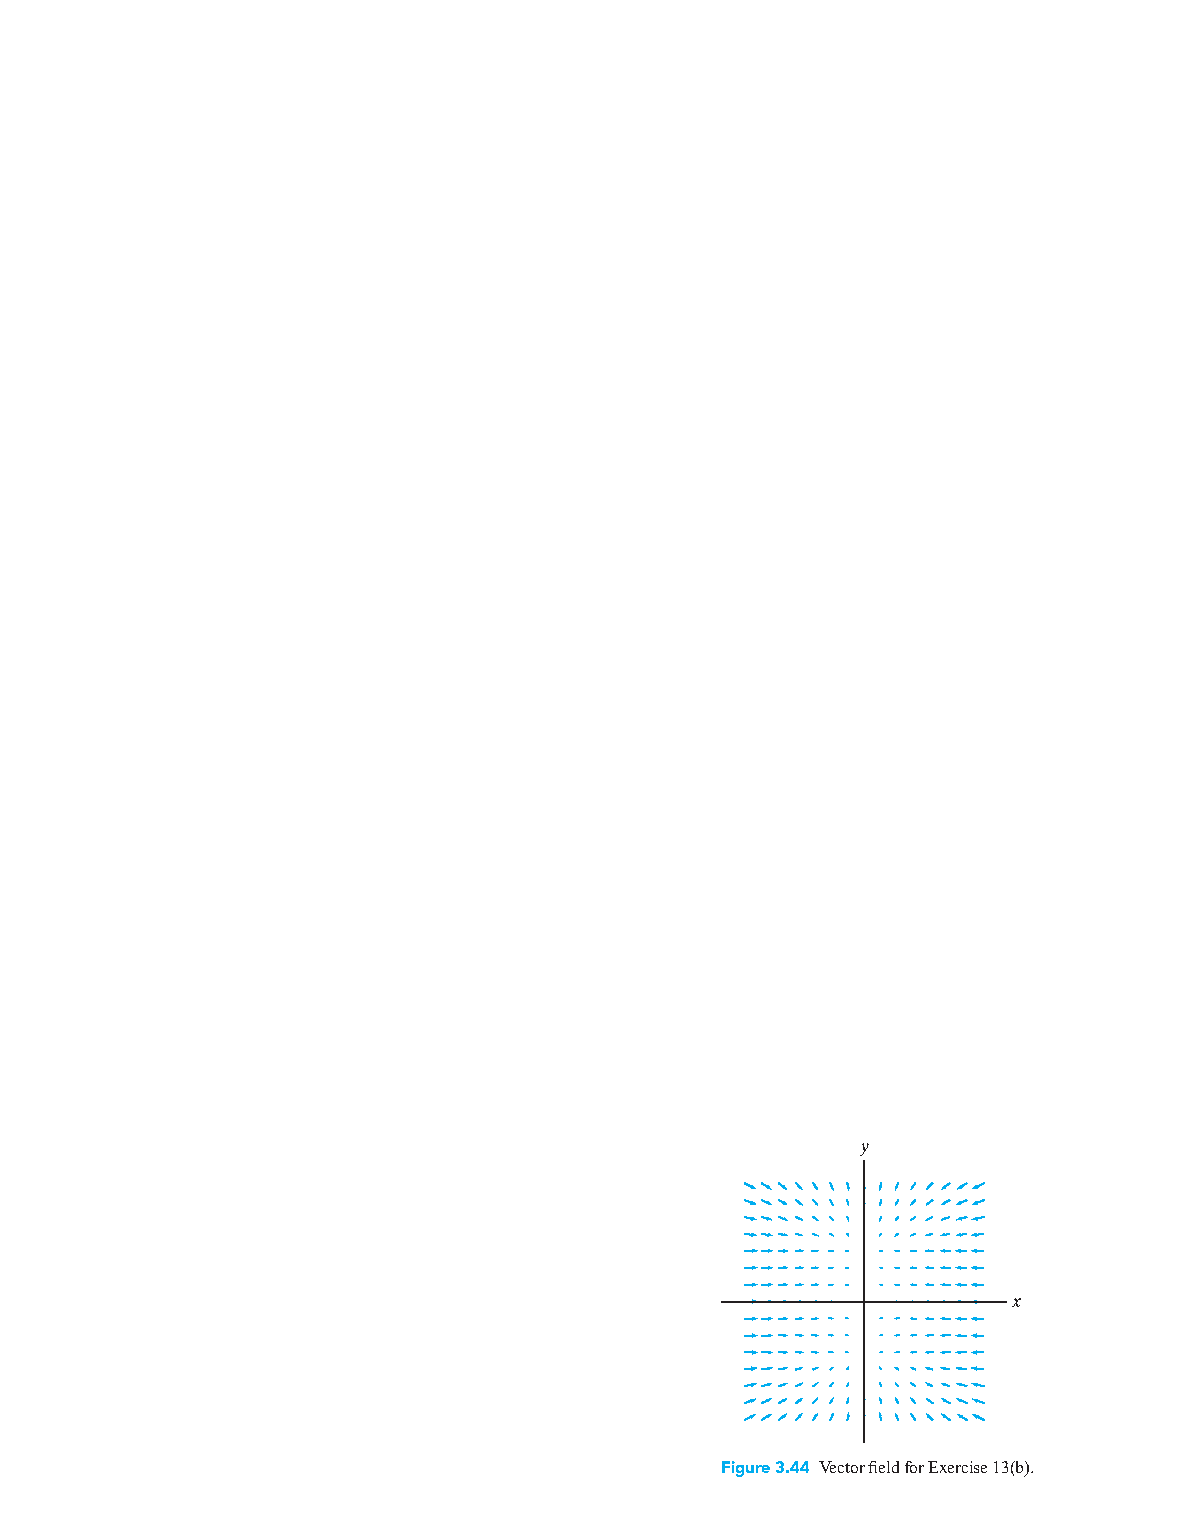
\includegraphics{img/3_4_13b}\\
		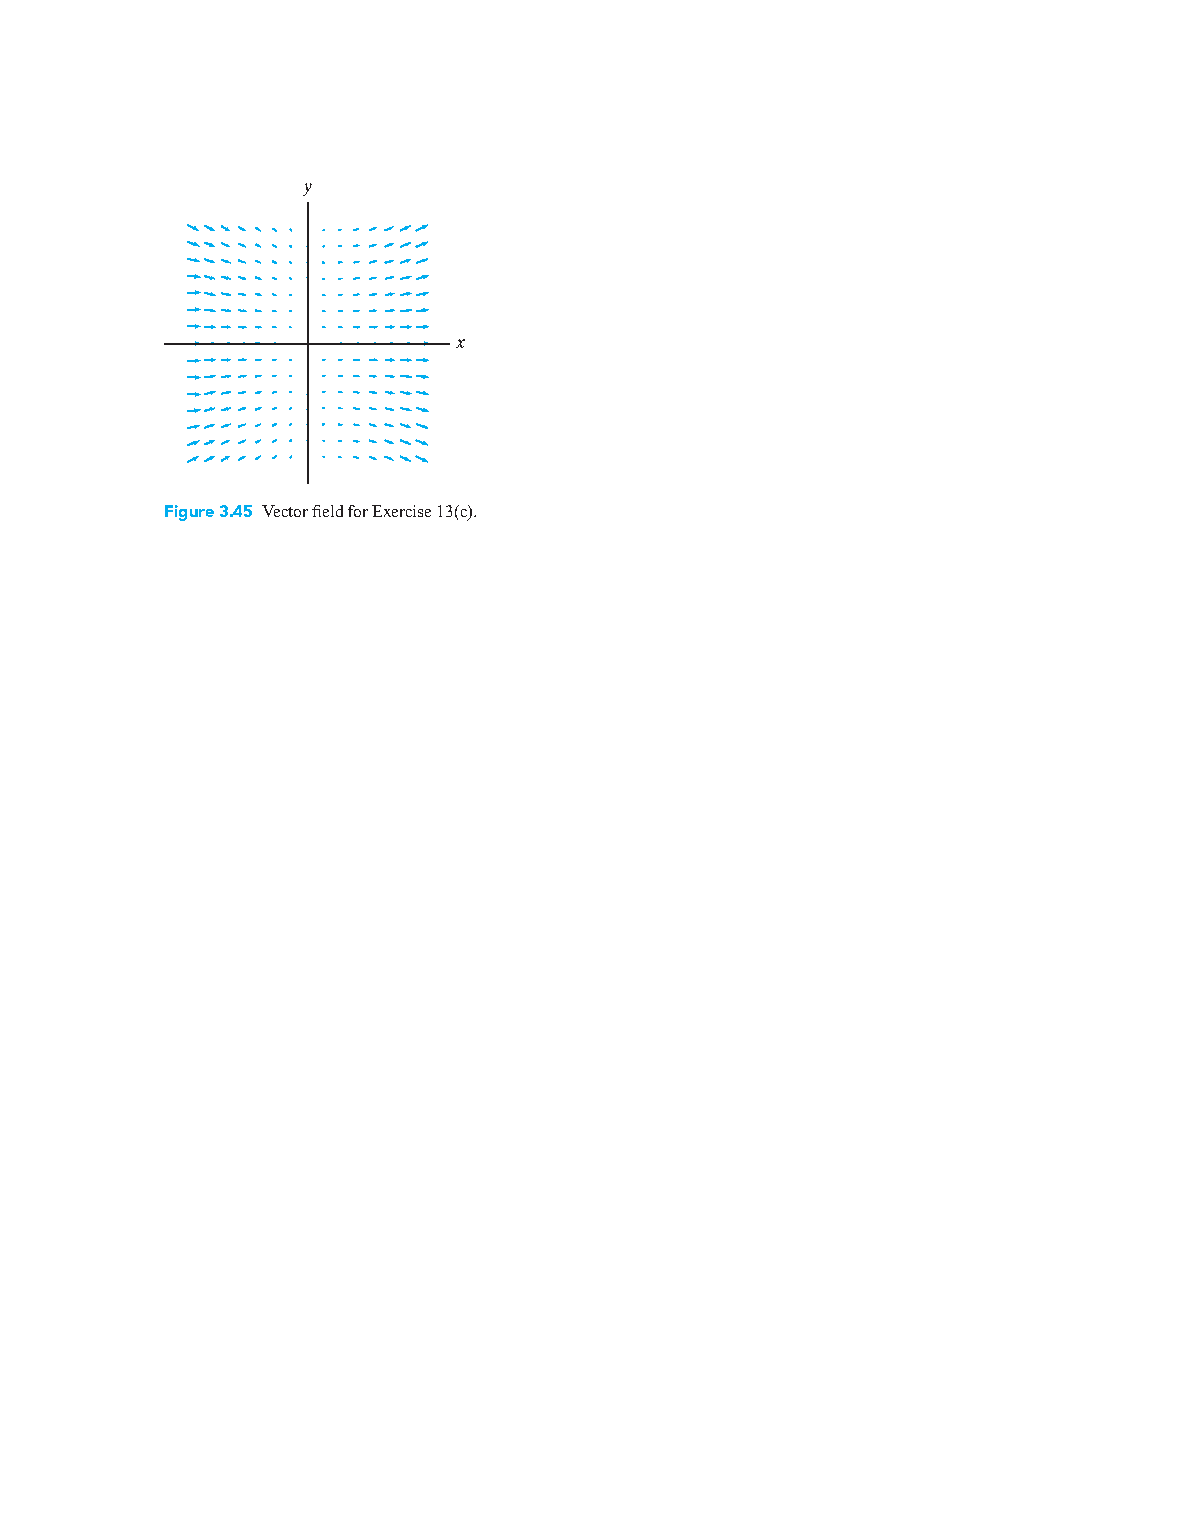
\includegraphics{img/3_4_13c}\qquad
		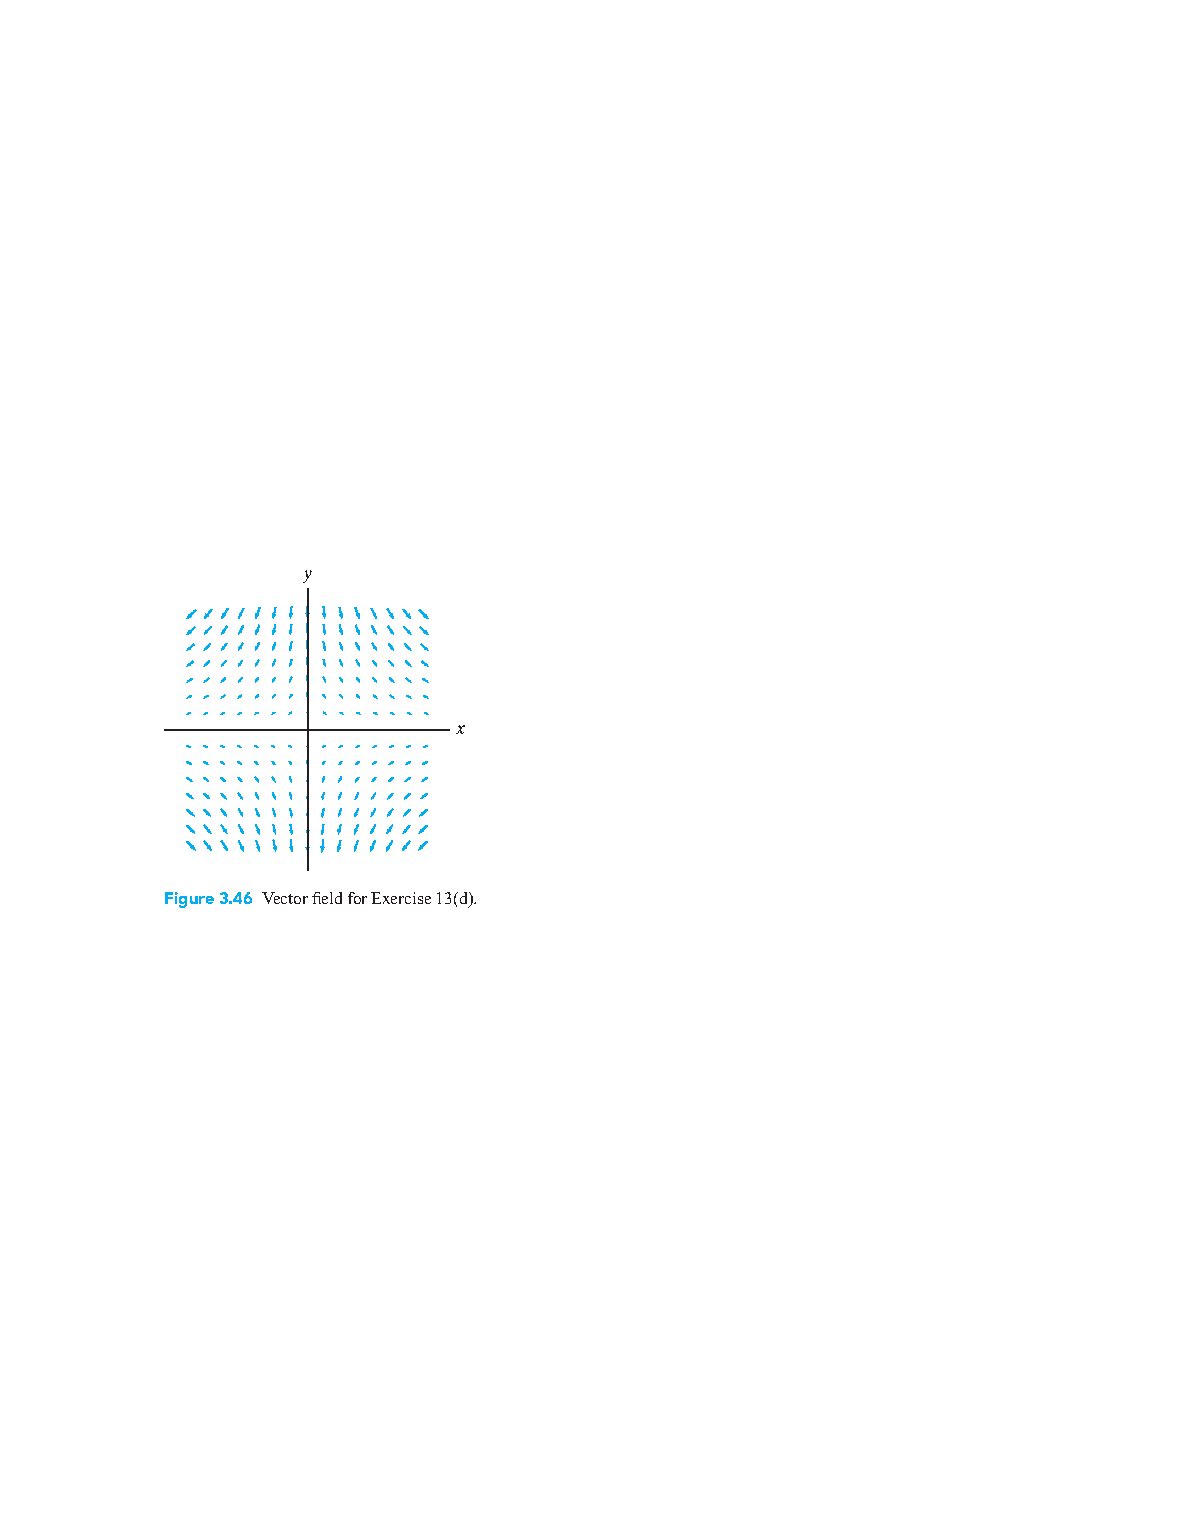
\includegraphics{img/3_4_13d}
	\end{center}
\end{problem}
\begin{solution}
	
\end{solution}

\begin{problem}[3.4.16]
	\fbox{\begin{minipage}{\linewidth}
		THEOREM 4.4:
		
		Let $\mathbf{F}: X \subseteq \mathbb{R}^3 \to \mathbb{R}^3$ be a vector field of class $C^2$.
		Then $\divergence(\curl F) = 0$. That is, $\curl F$ is an incompressible vector field.
	\end{minipage}}
	
	Prove Theorem 4.4.
\end{problem}
\begin{solution}
	
\end{solution}

\begin{problem}[3.4.23]
	Establish the given identity. 
	(You may assume that any functions and vector fields are appropriately differentiable.)
	\[
		\nabla\cdot(f\mathbf{F}) = f\nabla\cdot\mathbf{F} + \mathbf{F}\cdot\nabla f
	\]
\end{problem}
\begin{solution}
	
\end{solution}
\end{document}
